\chapter{Diseño e implementación}

En este capítulo se describirán las clases y todos los métodos que se han añadido y modificado durante el proceso de implementación a partir del código base de OpenBabel en su versión 3.1.1 (disponible en su repositorio oficial de GitHub\footnote{\url{https://github.com/openbabel/openbabel/releases}}). OpenBabel está escrito en C++, por lo que el proceso de desarrollo se ha llevado a cabo exclusivamente en este lenguaje, usando para ello el IDE \textit{Visual Studio C++} para Windows, (en el Anexo \ref{apend:manual} se detalla este proceso).


\section{Diseño}

\subsection{Estructura de OpenBabel}

A partir del código fuente de OpenBabel, al compilar los archivos fuente y generar el proyecto, los archivos de configuración de CMake generan una serie de \emph{soluciones}. Hay soluciones que consisten únicamente en el archivo `\textit{main}', que representa el ejecutable al que llamamos por línea de órdenes desde la terminal. El resto de soluciones forman la propia API de OpenBabel, siendo las clases más importantes `OBMol', `OBAtom', y `OBBond', que permiten almacenar la información de una molécula, un átomo, o un enlace entre átomos respectivamente; y otras clases más orientadas a la conversión entre formatos como `OBConversion' u `OBFormat'.

A continuación se muestra la estructura general de directorios de OpenBabel:
\vspace{0.5cm}
\dirtree{%
.1 openbabel-3-1-1/.
    .2 cmake/\DTcomment{\textit{algunos ficheros de configuración para cmake}}.
    .2 data/\DTcomment{}.
    .2 doc/\DTcomment{\textit{documentación del proyecto y ficheros para su generación automática}}.
    .2 include/\DTcomment{\textit{ficheros .h}}.
        .3 openbabel/.
            .4 depict/\DTcomment{\textit{representación de moléculas}}.
            .4 math/.
            .4 stereo/.
            .4 tree/.
            .4 clases principales de Openbabel.
                .5 ....
    .2 src/\DTcomment{\textit{ficheros .cpp}}.
        .3 charges/.
        .3 depict/\DTcomment{\textit{representación de moléculas}}.
        .3 descriptors/.
        .3 fingerprints/.
        .3 formats/\DTcomment{\textit{soporte para distintos formatos de conversión}}.
        .3 math/.
        .3 ops/\DTcomment{\textit{plugins de la comunidad}}.
        .3 stereo/.
        .3 clases principales de Openbabel.
            .4 ....
    .2 scripts/\DTcomment{\textit{bindings para usar la interfaz en otros lenguajes}}.
    .2 test/\DTcomment{\textit{ficheros de ejecución de tests y datos de prueba}}.
    .2 tools/\DTcomment{\textit{\textit{'mains'} para ejecución por línea de órdenes}}.
    .2 CMakeLists.txt\DTcomment{\textit{archivo principal de configuración de cmake}}.
    .2 INSTALL\DTcomment{\textit{instrucciones breves de instalación de openbabel}}.
    .2 ficheros propios de .git\DTcomment{}.
}


\subsection{Diagrama de Clases}

 En el siguiente Diagrama de clases (Figura \ref{fig:diagrama_clases}) se muestran tanto las clases que se han visto modificadas (en color anaranjado), las creadas desde cero (en color más verdoso) y las demás clases importantes que interactúan con las anteriores pero no se han visto alteradas (en amarillo). 

\begin{landscape}

    \begin{figure}[]
        \centering
        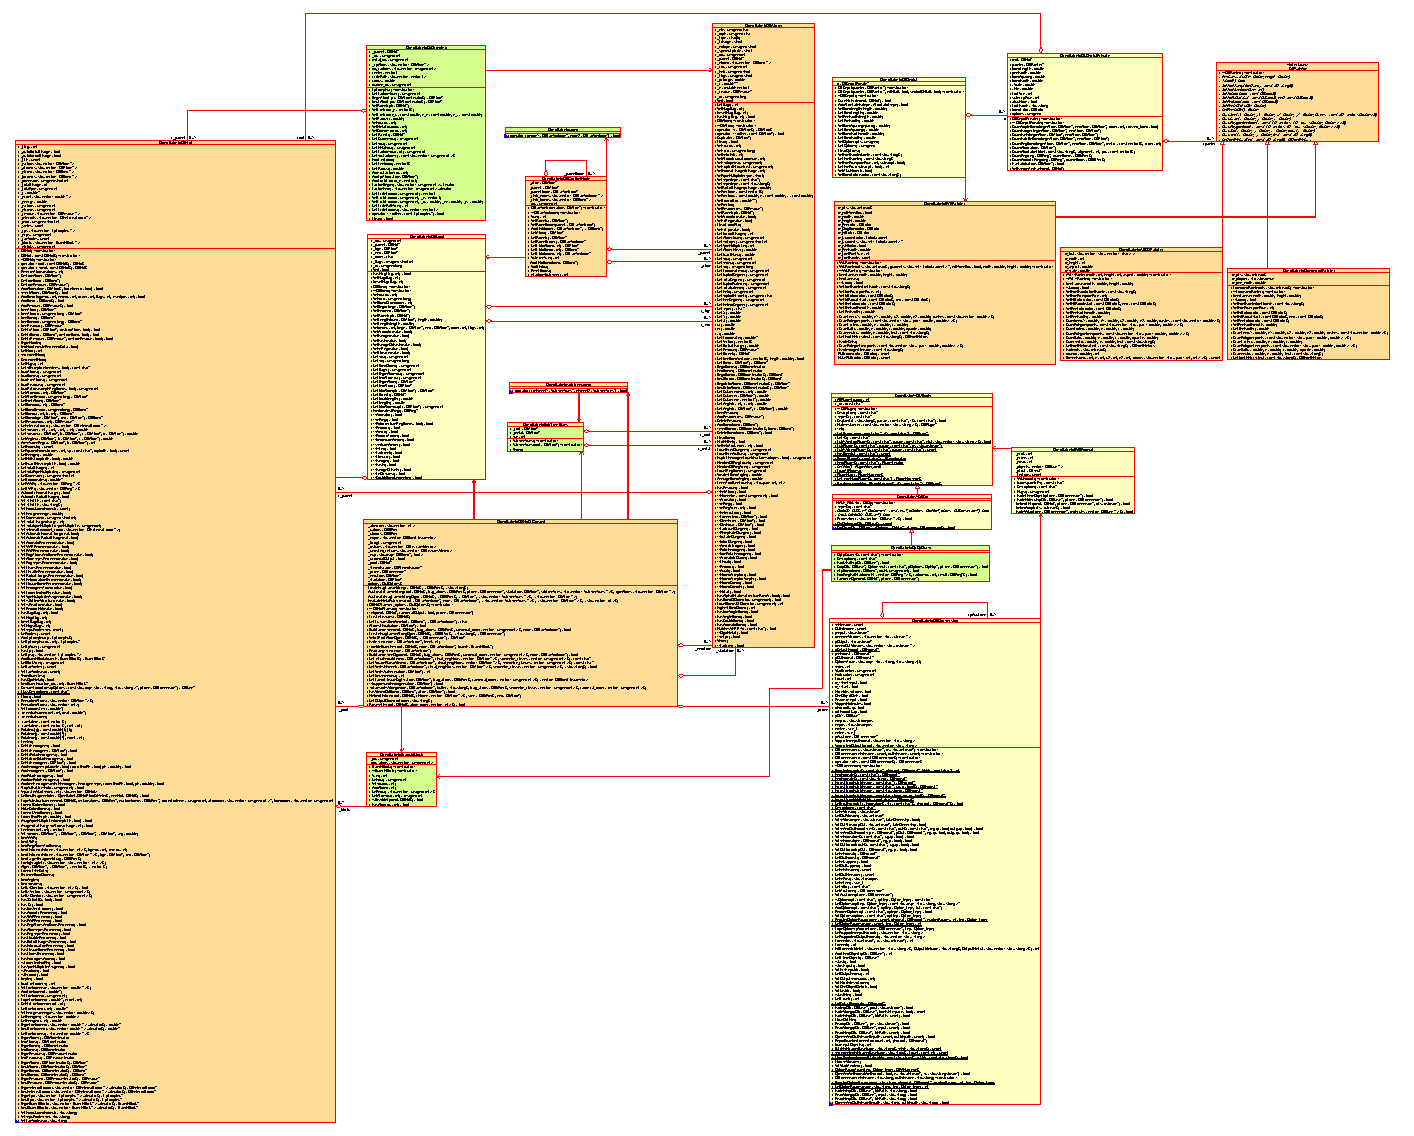
\includegraphics[scale=0.7]{imagenes/diseno/diagramaClasesHorizontal_cropped.pdf}
        \caption{Diagrama de clases}
        \label{fig:diagrama_clases}
    \end{figure}
\end{landscape}

% 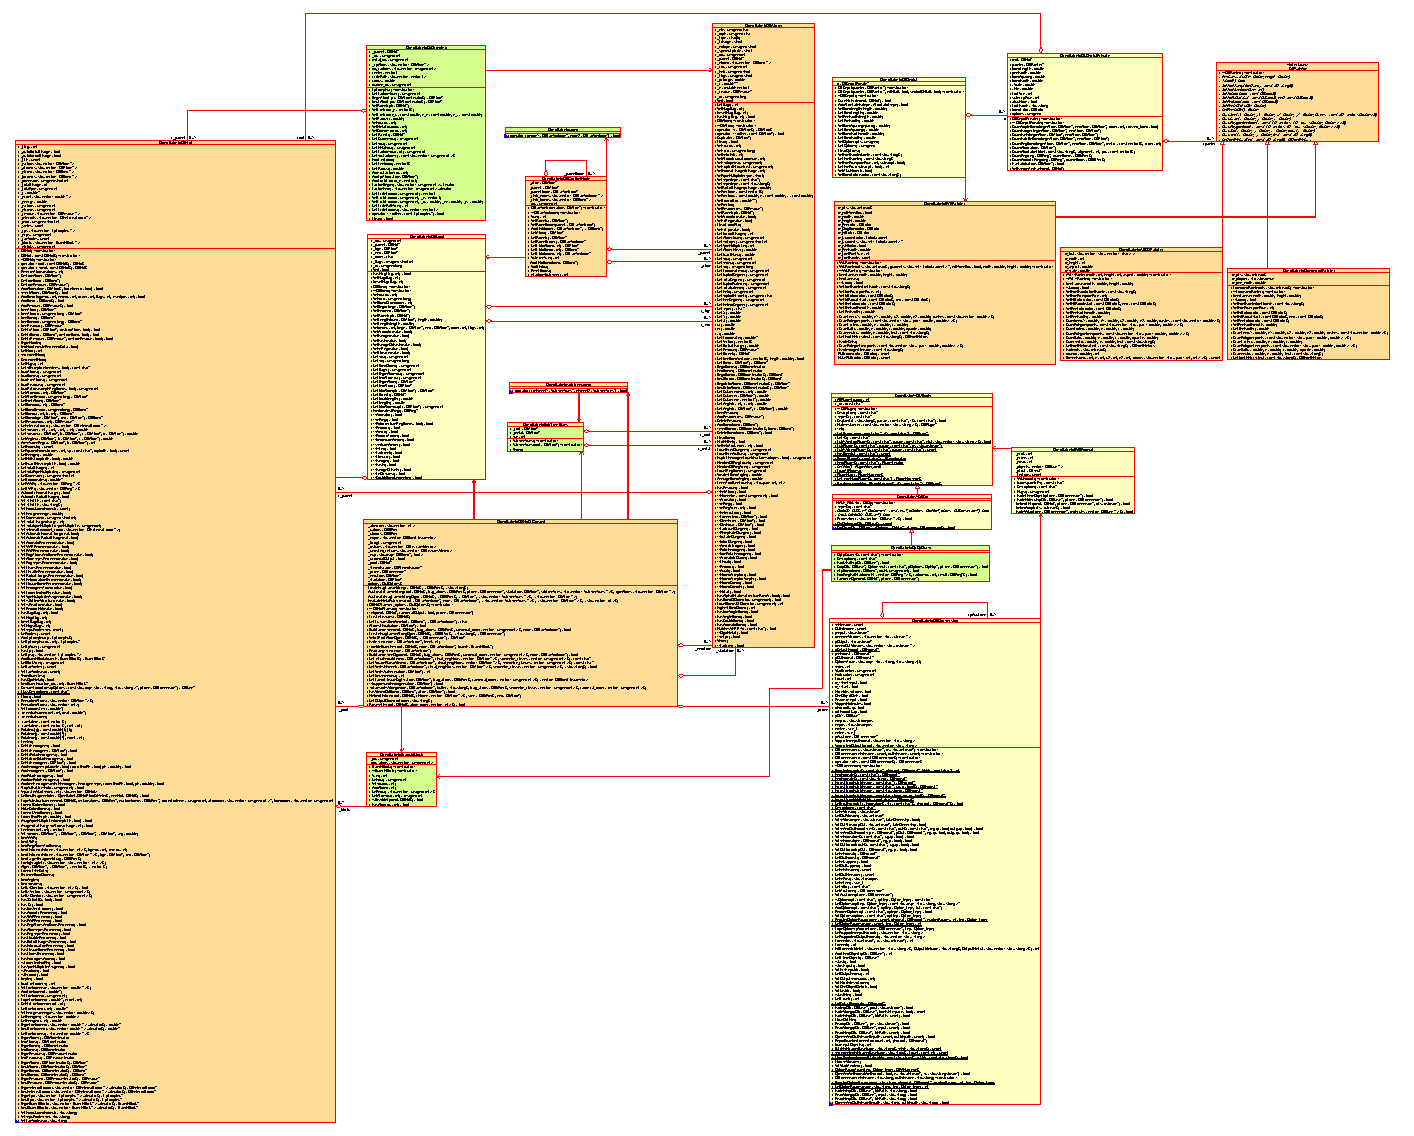
\includepdf[pages=-, offset=0 0,landscape=true,]{imagenes/diseno/diagramaClasesHorizontal_cropped.pdf}


Se pasa a detallar ahora cada una de las clases, tanto las modificadas como las nuevas, para qué sirven, y en qué consisten sus métodos. Las clases que no se han alterado, al igual que el resto de clases que no se incluyen en el diagrama se puede consultar su documentación en la página oficial\footnotemark. Puntualizar que existe una enorme cantidad de clases en la librería de OpenBabel, no tendería sentido añadirlas todas en el diagrama. Además, no todas poseen de documentación, por lo que la mayoría no aparecerán en\footnote[1]{\url{https://openbabel.github.io/api/3.0/index.shtml}}.


%  ------------------------- Cabeceras -------------------------
\subsection{Clases modificadas}
\begin{itemize}
    \item \textbf{OBPainter}: clase base abstracta para las clases de representación gráfica 2D (en \textit{/depict/painter.h}). Se ha añadido el siguiente método para poder utilizarlo en las clases que implementan esta interfaz:
    \begin{lstlisting}[language=C++]
        public: 
    
virtual void DrawPolygonLine(const std::vector<std::pair<double, double> >& points) = 0;
    \end{lstlisting}

    \item \textbf{SVGPainter}: clase que hereda de OBPainter y genera representaciones 2D en el formato de gráficos vectoriales SVG (en \textit{/depict/svgpainter.h}).
    \begin{lstlisting}[language=C++]
        public: 
    
//Inserts the necessary xml code in the .svg output file to draw a polygon according to the vector of points specified by @p points
void DrawPolygonLine(const std::vector<std::pair<double, double> >& points);
    \end{lstlisting}

    \item \textbf{ASCIIPainter}: clase que hereda de OBPainter (en \textit{/depict/asciipainter.h}).
    \begin{lstlisting}[language=C++]
        public: 
    
//The method is declared empty to avoid compilation errors due to interface implementation. It has no use 
void DrawPolygonLine(const std::vector<std::pair<double, double> >& points);
    \end{lstlisting}

    \item \textbf{CommandPainter}: clase que hereda de OBPainter (en \textit{/depict/commandpainter.h}).
    \begin{lstlisting}[language=C++]
        public: 
    
//The method is declared empty to avoid compilation errors due to interface implementation. It has no use 
void DrawPolygonLine(const std::vector<std::pair<double, double> >& points);
    \end{lstlisting}

    % -------------------------- Atom ---------------------------
    \item \textbf{OBAtom}: clase principal, contiene la información relativa a un átomo, guardando su número atómico, cantidad de hidrógenos implícitos, una lista de los enlaces de este átomo con los demás y el vector de coordenadas 2D para su representación, entre otras variables (en \textit{/openbabel/atom.h}). Se han añadido los siguientes métodos:
    \begin{lstlisting}[language=C++]
class OBAPI OBAtom: public OBBase{
    public: 
    
//\return Is this a metal commonnly present in organometallic compounds?
bool IsOgmMetal();

//\return Is atom part of a Cp ring?
bool IsInCp() const;

//\return Is this atom a Carbon (atomic number == 6)?
bool IsCarbon();

//Debug method. Displays on basic output simple data to identify the atom
void Show();

//Mark an atom as part of a Cp ring
void SetInCp(bool value = true);
};//class
    \end{lstlisting}


    % -------------------------- Mol ---------------------------
    \item \textbf{OBMol}: clase principal, almacena toda la información básica relacionada con una molécula. Esto incluye la lista de átomos, la lista completa de enlaces entre átomos, identificadores de los átomos y enlaces, y el vector de coordenadas 2D de todos los átomos para su representación entre otras variables (en \textit{/openbabel/mol.h}). Se han añadido las siguientes variables y métodos:
    \begin{lstlisting}[language=C++]
class OBAPI OBMol: public OBBase {
    private: 
    
std::string _smiles;                //!< Input smiles string for the molecule
std::vector<CpComplex*> _cps;       //!< Cp information
unsigned int _ncps;                 //!< Number of cps complexes detected
std::string  _canSmiles;            //!< Canonical smiles based on Ogm canonicalization
std::vector<BranchBlock*> _blocks;  //!< Branches information
unsigned int _nblocks;              //!< Number of blocks


    public: 
    
//! Set the input smiles string of this molecule to @p smi
void SetInputSmiles(std::string smi);

//! \return the input smiles string of this molecule
std::string GetSmiles();

//! Add a new CpComplex specified by @p cp
void AddCpComplex(CpComplex& cp);

//! \return the cp at index @p idx or NULL if none exists.
CpComplex* GetCpComplex(int idx);

//! \return number of cp in the molecule
unsigned int GetCpSize();

//! \return whether the molecule has cps or not
bool HasCp();

//! \return the whole container of cps of this molecule
std::vector<CpComplex*> GetCps();

//! Add a new block to the molecule, specified by @p branch
BranchBlock* AddBranchBlock(BranchBlock& branch);

//! \return the number of blocks in the molecule
unsigned int GetBlockSize();

//! \return the canonical smiles string generated by the ogm canonicalization methods
std::string GetCanSmiles();

//! Set the canonical smiles string of this molecule to @p smi
void   SetCanSmiles(std::string smi);

//! Debug method. Displays on basic output all molecule blocks with basic information of the atoms.
void ShowBranches();

//! \return If this molecule has any Ogm metal or not
bool HasOgmMetal();

//! \return the block of which the carbon at index @p carbon_idx is part, or NULL if no such block exists
BranchBlock* FindBranch(int carbon_idx);

//! Set the iterator to the beginning of the Cp list
//! \return the first Cp structure, or NULL if none exist
CpComplex* BeginCp(std::vector<CpComplex*>::iterator & i);

//! Advance the iterator to the next Cp record
//! \return the next first Cp record, or NULL if none exist
CpComplex* NextCp(std::vector<CpComplex*>::iterator& i);

//! Set the iterator to the beginning of the BranchBlock list
//! \return the first BranchBlock structure, or NULL if none exist
BranchBlock* BeginBranchBlock(std::vector<BranchBlock*>::iterator& i);

//! Advance the iterator to the next BranchBlock record
//! \return the next first BranchBlock record, or NULL if none exist
BranchBlock* NextBranchBlock(std::vector<BranchBlock*>::iterator& i);
};//class
    \end{lstlisting}


    % -------------------------- OBMol2Cansmi ---------------------------
    \item \textbf{OBMol2Cansmi}: clase que maneja la conversión del smiles de entrada a un smiles canónico (en \textit{src/formats/smilesformat.h}). Se han añadido los siguientes métodos:
    \begin{lstlisting}[language=C++]
class OBMol2Cansmi{
        private: 
    
//Only changed visibility to private, since CreateFragCansmiStringOgm was created. Selects the "root" atom, which will be first in the SMILES, then builds a tree in canonical order, and finally generates the SMILES.
void CreateFragCansmiString(OBMol&, OBBitVec&, std::string&);

    
//Auxiliary private methods for SelectRootAtomOgm

//Shortened version of the CreateCansmiString method. Create the necessary variables to call AuxCreateFragCansmiStringOgm.
void AuxCreateCansmiString(OBMol& mol, OBBitVec& frag_atoms, OBConversion* pConv, OBAtom* startatom, std::vector<SubTreeSizes*>& subtreeSizes, std::vector<OBAtom*> ogmAtoms);

//Shortened version of the CreateFragCansmiStringOgm method. Create the necessary variables to build a new canonical tree using as root @p startAtom
void AuxCreateFragCansmiStringOgm(OBMol&, OBBitVec&, OBAtom*, std::vector<SubTreeSizes*>&, std::vector<OBAtom*>);

//Once the tree is built, this method runs through it in DFS evaluating the subtrees hanging from the other ogm metals. Use the auxiliary struct SubTreeSizes for this. 
void EvaluateMetalSubTrees(OBCanSmiNode* root, OBCanSmiNode* node, std::vector<SubTreeSizes*>&, std::vector<OBAtom*>&, std::vector<int>&);

        public: 
//Method based on CreateFragCansmiString. Share much of the code, with some additional methods specifically for my own canonical form designed for organometallic molecules.
void CreateFragCansmiStringOgm(OBMol&, OBBitVec&, std::string&, OBConversion*);

//If more than 1 Ogm metal is present in the molecule, this method chooses one of them, based on some rules and the conectivity of the metal within the molecule and the rest of the atoms
OBAtom* SelectRootAtomOgm(OBMol&, OBConversion*);

//Debug method for writing in basic output the tree with hierarchy formating
void WriteTree(OBCanSmiNode* node, int level = 0);

//Adds information to the molecule of the blocks that form it. Being a block, each set of atoms that, due to their bonds, are within the same parenthesis in the original input Smiles. Or, according to the OBMol2Cansmi::BuildCanonTree method, the parent-child relationship between atoms.
void IdentifyBranches(OBMol& mol,OBCanSmiNode* node, BranchBlock* branch = nullptr);

//Modifies the tree built by BuildCanonTree based on the length of the branches identified in IdentifyBranches. This is a canonical rule designed for a little more consistency in the output canon smiles.
void RearrangeTree(OBCanSmiNode* node);

//Builds the SMILES tree, in canonical order, for the specified molecular fragment. Based on the BuildCanonTree method. Shares much of the code, with some changes in the neighbour selection algorithm.
bool BuildCanonTreeOgm(OBMol& mol, OBBitVec& frag_atoms, vector<unsigned int>& canonical_order, OBCanSmiNode* node);
};//class
    \end{lstlisting}


    % -------------------------- OBCanSmiNode ---------------------------
    \item \textbf{OBCanSmiNode}: clase que representa un nodo. En conjunto se forma una estructura de árbol, cada nodo es un átomo del árbol para luego escribir el SMILES canónico (en \textit{src/formats/smilesformat.h}). Se han añadido los elementos:
    \begin{lstlisting}[language=C++]
class OBMol2Cansmi{
        private: 
    
OBCanSmiNode* _parentNode;      //!< Pointer to the parent node

//! Add a child bond to the node, specified by @p bond. Should only be used in the ResetBonds method as a part of the OBMol2Cansmi::RearrangeTree algorithm.
//! Otherwise, use addChildnode to add both the child node and its respective bonds
void AddChildBond(OBBond* bond);

        public: 

//! Set the parent node to @p parent
void SetParentNode(OBCanSmiNode* parent);

//! \return the parent node
OBCanSmiNode* GetParentNode();

//! Traverses the tree in dfs from the node calling the method
//! \return the number of total children (counting himself) 
int SubTreeSize();

//! Sort a node's child_nodes using a std::sort operation an a custom comparator 'mycomp'
void SortChilds();

//! When added at the same time in the addchildnode method, the child with its bond have a 1 to 1 index correspondence. When reordering the children, in OBMol2Cansmi::RearrangeTree, the indices of the bonds are lost. This method clears and adds the bonds back in order.
void ResetBonds();

//! \return the total number of carbons in this node subtree
int nCarbonsSubTree();
};//class
    \end{lstlisting}

\end{itemize}





\subsection{Clases nuevas}
\begin{itemize}
    % -------------------------- CpComplex ---------------------------
    \item \textbf{CpComplex}: nueva clase principal que maneja y permite almacenar estructuras de ciclopentadienilo (en \textit{/openbabel/cpcomplex.h}). Se han creado las siguientes variables y métodos:
    \begin{lstlisting}[language=C++]
class CpComplex {
	protected:
  
OBMol* _parent;                         //!< Parent molecule
unsigned int _idx;                      //!< Cp identifier within the molecule
unsigned int metal_idx;                 //!< Atom idx of central metal
std::vector<OBAtom*> _cpAtoms;          //!< Atoms for the carbons of the Cp structure
std::vector<unsigned int> idx_carbons;  //!< Atom indexes for the carbons of the Cp structure
vector3 center;                         //!< Cp center, for normal bond connection with metal atom, and aromatic circle position
std::vector<vector3> circlePath;        //!< Coordinates for the cp circle (needed to achieve a perspective circunference)
double radius;                          //!< Cp's aromatic circle radius
unsigned int dummy_idx;                 //!< Dummy central atom idx


        public:

//! Default constructor 
CpComplex();

//! \name Methods to modify internal information
//@{
//! Attach an OBMol @p ptr as the parent container for this Cp
void SetParent(OBMol* ptr);
//! Set the center point of the Cp, sprecified by @p _v. It is equidistant to every carbon in th Cp, as they are disposed in a regular polygon
void SetCentroid(vector3& _v);
//! Set the center point of the Cp, sprecified by @p v_x, v_y, v_z. It is equidistant to every carbon in th Cp, as they are disposed in a regular polygon
void SetCentroid(const double v_x, const double v_y, const double v_z);
//! Set the radius of the Cp circle
void SetRadius(double r);
//! Set the Cp identifier
void SetIdx(int idx);
//! Set the idx of the central metal to which this Cp is attached
void SetMetalIdx(int midx);
//! Dummy atom is created to make a perpendicular bond between the metal and the Cp drawing
//! Set the atom idx of the dummy atom created for this Cp 
void SetDummyIdx(int idx);
//! Set the point of the Cp circle at index @p i to the coordinates specified by @p _v
void SetCircleCoord(unsigned int i, vector3 _v);
//! Set the point of the Cp circle at index @p i to the coordinates specified by @p _vx, _vy, _vz
void SetCircleCoord(unsigned int i, double _vx, double _vy, double _vz = 0.0);
//@}


//! \name Methods to retrieve information
//@{
//! \return number of carbon atoms in the cp
unsigned int GetCarbonsSize();
//! \return the molecule which contains this Cp, or NULL if none exists
OBMol* GetParent();
//! \return dummy atom idx for this Cp structure, or 0 if none exists
unsigned int GetDummyIdx() const;
//! \return Cp identifier
unsigned int GetIdx() const;
//! \return Central metal identifier
unsigned int GetMetalIdx() const;
//! \return carbon idx at position @p i in tha container. Zero based access method to vector
unsigned int GetCarbonIdx(int i) const;
//! \return the whole contanier of carbon idx
const std::vector<unsigned int>& GetIdxCarbons();
//! \return the centroid of this Cp in a coordinate vector
vector3& GetCentroid();
//! \return the radius of the Cp circle
double GetRadius();
//! \return the coordinate vector for the Cp circle point at position @p i in the container. Zero based access method to vector
vector3 GetCircleCoord(unsigned int i);
//! \return the number of points of the Cp circle
int GetCirclePathSize() const;
//! \return the whole container of coordinates of the Cp circle
std::vector<vector3> GetCircleCoords() const;
//@}


//! \name Addition of data for a Cp
//@{
//! Adds a new atom idx to this Cp
void AddIdxCarbon(int idx);
//! Adds a new atom to this Cp
void AddCpAtom(OBAtom* atom);
//! Adds a new point to the coordinate vector that forms the Cp circle
void AddCircleCoord(vector3 _v);
//@}


//! \name Iteration methods
//@{
//! Set the iterator to the beginning of the Cp atom list
//! \return the first atom, or NULL if none exist
OBAtom* CpComplex::BeginAtomCp(OBAtomIterator& i);
//! Advance the iterator to the next atom in the Cp
//! \return the next first atom record, or NULL if none exist
OBAtom* CpComplex::NextAtomCp(OBAtomIterator& i);
//@}


//! \name Other operations
//@{
//! Calculate and set the centroid of this Cp, taking into consideration all atoms stored in _cpAtoms
void FindCentroid();
//! Equivalence operator
bool operator==(const CpComplex* other) const;
//@}
};//class
    \end{lstlisting}


    % -------------------------- BranchBlock ---------------------------
    \item \textbf{BranchBlock}: clase que representa un grupo funcional aislado dentro de la molécula, p.ej. un ciclo de benceno, un Cp, o toda una rama de un átomo (en \textit{/openbabel/cpcomplex.h}). Se han añadido las siguientes variables y métodos:
    \begin{lstlisting}[language=C++]
class BranchBlock {
        private: 
    
unsigned int _idx;                          //!< Block identifier
std::vector<unsigned int> vidx_atoms;       //!< Vector idx of the atoms that are part of the block.

        public: 

//! Default constructor
BranchBlock();

//! Destructor
~BranchBlock();

//! \return the size of the block (number of atoms in the block)
int Size();

//! \return the block identifier
unsigned int GetIdx();

//! Set the block identifier
void SetIdx(int idx);

//! Add an atom's idx to the block
void AddAtom(int i);

//! \return the idx of the atom at position @p i. Zero based access.
unsigned int GetAtomIdx(int i);

//! \return Whether the @p idx exists within the atoms already inserted in the block
bool HasAtom(int idx);

//! Cp will be possible if all the elements in the block are carbons up to that point and have a bond with an ogm metal.
//! \return whether or not it appears to be a Cp block
bool IsPossibleCp(OBMol &mol)
}; //class
    \end{lstlisting}


    % -------------------------- OpCpDraw ---------------------------
    \item \textbf{OpCpDraw}: clase plugin que hereda de OBOp (en \textit{/ops/cpdraw.cpp}). Contiene el algoritmo de detección, identificación, y almacenamiento en la molécula de estructuras tipo Cp.
    \begin{lstlisting}[language=C++]
class class OpCpDraw : public OBOp {
//! Default constructor
OpCpDraw(const char* ID);

//! Inherited method. 
//! Display through the output stream a brief description of the plugin.
const char* Description();

//! Inherited method. 
//! \return true if this op (plugin operation) is designed to work with the class of @p pOb, e.g. OBMol
virtual bool WorksWith(OBBase* pOb) const;

//! Inherited method. Required function that does the work. Normally return true, unless object is not to be output. 
virtual bool Do(OBBase* pOb, const char* OptionText = nullptr, OpMap* pOptions = nullptr, OBConversion* pConv = nullptr);

//! \return If @p bond is likely to be a cp-bond like
bool isCpBond(OBBond* bond, unsigned int idxM);

//! Finds the ring of which the carbon with idx @p carbonIdx is a part of, among the rings of @p rlist (obtained from a SSSR perspective), and stores it in @p result.
//! \returns whether it was found or not
bool FindRingWithCarbon(vector<OBRing*>& rlist, int carbonIdx, OBRing*& result);

//! Canonize the input SMILES and identify blocks
void CanonizeOgm(OBMol* mol, OBConversion* pConv); 
}; //class
    \end{lstlisting}


    
    % -------------------------- SubTreeSizes ---------------------------
    \item \textbf{SubTreeSizes}: struct auxiliar creado para la selección del primer metal durante la canonización (se profundiza sobre esto en la Sección \ref{canonizacion}). Contiene las siguientes variables y métodos (en \textit{src/formats/smilesformat.h}):
    \begin{lstlisting}[language=C++]
struct SubTreeSizes {

OBAtom* _root;      //!< Tree root
OBAtom* _metal;     //!< Metal to evaluate
int size;           //!< Size of the subtree for the _metal to evaluate
int nCarbons;       //!< Number of carbon atoms

//! Default constructor
SubTreeSizes();

//! Parameter constructor. Creates a new object with _root as @p root
SubTreeSizes(OBAtom* root);

//! Debug method. Displays through basic output the struct information.
void Show();
};//struct
    \end{lstlisting}


    % -------------------------- subtreecomp ---------------------------
    \item \textbf{subtreecomp}: objeto comparador que prioriza unos metales sobre otros en el proceso de selección del átomo raíz para el árbol (en \textit{src/formats/smilesformat.h}).
    \begin{lstlisting}[language=C++]
struct subtreecomp {
bool operator() (SubTreeSizes* element1, SubTreeSizes* element2) const;
}subtreecomp;
    \end{lstlisting}


    % -------------------------- mycomp ---------------------------
    \item \textbf{mycomp}: objeto comparador que prioriza las ramas del árbol canónico durante el proceso de reordenación (en \textit{src/formats/smilesformat.h}).
    \begin{lstlisting}[language=C++]
struct comp{
bool operator() (OBCanSmiNode* node1, OBCanSmiNode* node2);
}mycomp;
    \end{lstlisting}
    
\end{itemize}


En resumen, se han modificado 8 clases existentes, sufriendo los cambios más importantes las clases OBMol, OBAtom, OBCanSmiNode y OBMol2Cansmi; y se han añadido 6 clases nuevas. En total, se han agregado 93 métodos y 22 variables nuevas. Con todo esto, en la siguiente sección se describen los algoritmos implementados.

\section{Implementación}

\subsection{Nomenclatura canónica} \label{canonizacion} \label{implementacion:canonizado}

La idea detrás de una canonización, como ya se ha comentado, es obtener una representación única para una molécula independientemente de su forma inicial. Para ello se suelen emplear estructuras de tipo árbol y realizar un recorrido de los nodos de una forma concreta. La información de la que disponemos para una molécula tras un proceso de parsing de la cadena SMILES de entrada, es una lista de átomos y una lista de enlaces entre átomos. Estas estructuras de datos lineales se utilizan para generar el árbol, donde los nodos serán los átomos y las aristas los enlaces. OpenBabel almacena esta estructura de datos a través de la clase \textit{OBCanSmiNode}, que representa cada nodo individual y contiene: el átomo del nodo, el átomo del nodo padre, un vector con los nodos hijos y un vector con los enlaces a los hijos.

El SMILES de salida dependerá por tanto de 2 factores. Primero, el orden en el que se recorra el árbol, que dado nuestro objetivo de obtener un canónico, el recorrido será siempre el mismo. En este caso OpenBabel utiliza un recorrido en profundidad de preorden (DFS, Depth First Search en inglés). Y segundo, aunque el recorrido sea el mismo, si el árbol cambia, el resultado será distinto. Por lo que se debe ser capaz de generar consistentemente el mismo árbol si la molécula es la misma. Con ese propósito se le asigna a cada nodo una etiqueta (label) única, independientemente de su orden de entrada, para luego a la hora de generar el árbol saber qué átomos tienen preferencia sobre otros. Este algoritmo de asignación de etiquetas es lo que suele diferenciar unos toolkits de otros.

En el estado actual, OpenBabel cuenta con su propio algoritmo de canonización en 2 versiones. Ambas por defecto realizan un tratamiento de ciclos, colocándolos en su forma aromática y reutilizando los números de apertura y cierre, pero se diferencian en la asignación de las etiquetas. Hay una versión canónica simple (\textit{standard labels}) en la que se asignan las etiquetas en orden ascendente de llegada, del 0 al $n$ siendo $n$ el número total de átomos en la molécula. Por tanto, el SMILES canónico resultado no varía en nada respecto al SMILES de entrada excepto por el tratamiento de los ciclos. 

Y una versión canónica completa (\textit{canonical labels}) basada en el algoritmo de Morgan y en el uso de los invariantes de un átomo \cite{vogt_powerpoint, apodaca_computing_2019}. Estos invariantes son características únicas que clasifican a cada átomo en base a: su topología con respecto a los demás átomos en el grafo molecular, el número de conexiones, cantidad de hidrógenos enlazados, número atómico, carga eléctrica, etc. El algoritmo en sí mismo es bastante complejo, por lo que no se tratará más en profundidad. Para más detalles de su implementación y trasfondo ver \cite{weininger_smiles_1989, canonical_coding_algorithm, jochum_canonical_1977, vogt_powerpoint}. 

Para el objetivo del proyecto nos sirve con saber que dicho algoritmo proporciona buenos resultados y el uso de las \textit{canonical labels} funciona adecuadamente para todas las moléculas, en el sentido de que las hace canónicas. Es efectivo también para moléculas organometálicas, pero no le da la suficiente importancia al metal. El sistema de canonización propuesto en este proyecto está basado en las peticiones de la experta. Siguiendo sus recomendaciones, les sería útil que en compuestos organometálicos el SMILES comenzara por el metal. En la Figura \ref{fig:canonicos_mal_implementacion}, se muestran algunos ejemplos de moléculas organometálicas canonizadas usando los \textit{canonical labels}. Vemos que el metal se encuentra siempre enmarañado por medio del SMILES rodeado de otros enlaces que pueden ser o no ser suyos, entorpeciendo el ver qué conectividad tiene dicho metal. 

\begin{figure}[h!]
    \centering
    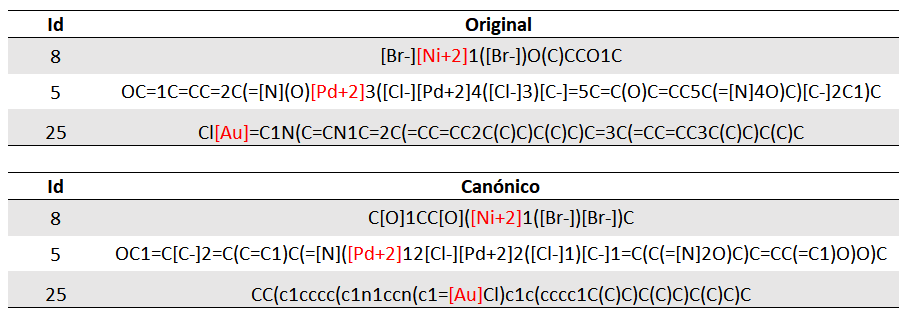
\includegraphics[scale=0.5]{imagenes/diseno/canonizado/canonicos_mal_implementacion.png}
    \caption{SMILES canónicos pertenecientes a la organometálica según el algoritmo propio de OpenBabel. Los metales están marcados en rojo. Son 3 moléculas del dataset mostrado en el Anexo \ref{apend:pagina_tabla_intro_grande}, identificadas por su Id.} 
    \label{fig:canonicos_mal_implementacion}
\end{figure}



\subsubsection{Reglas canonizado} \label{reglas_canonizado}

Se busca por tanto, lo primero de todo colocar el metal al inicio del SMILES y en base a esto ir colocando el resto de átomos vecinos. Esto también se cree que sería beneficioso a la hora de trabajar con modelos generativos. El tener una estructura legible y estricta en donde se fije el metal al principio de la cadena favorece la robustez de la representación \cite{SELFIES, krenn_self_referencing_2020}.
En base a la premisa de colocar el metal lo primero, se ha desarrollado un sistema canónico con las siguientes reglas:
\begin{itemize}
    \item Tiene que haber un metal de interés para la organometálica (los metales de transición mencionados en la Sección \ref{teoria:ogm}) en el SMILES de entrada para aplicar el algoritmo de canonizado propio. En caso negativo, se aplicaría el original de OpenBabel. 
    \item Si el SMILES está desconectado (por fragmentos) se aplicará el algoritmo original. El SMILES resultado es la concatenación de cada fragmento canonizado por separado.
    \item Para escoger el metal que da inicio al SMILES se siguen las siguientes prioridades:
        \begin{enumerate}
            \item Si solamente hay un metal, se escoge dicho átomo directamente.
            \item Si hay más de 1 metal, se selecciona el que tiene mayor cantidad de subhijos (mayor tamaño de su subárbol) con respecto a los demás metales. Se considera que el metal más importante es del cuál dependen más átomos. Para esto se generan 
            \item Si la condición anterior resulta en empate, se toma el metal con mayor número atómico.
            \item Si la condición anterior resulta en empate, es decir, es el mismo elemento con la misma cantidad de subhijos, se toma el metal que de entre sus subhijos aparezcan menos carbonos. Ya que los carbonos son esenciales, son muy frecuentes. Por lo que se da prioridad a cualquier otro elemento antes.
            \item Si lo anterior también resulta en empate, todo indica que se trata de una molécula simétrica, por lo que no importa qué metal se escoja.
        \end{enumerate}
\end{itemize}

Se esboza a continuación un pseudo código en lenguaje natural que muestra el flujo de ejecución del método principal, \textit{CreateFragCanSmiStringOgm}, durante la canonización. 
\begin{algorithm}[h!]
   \caption{CreateFragCanSmiStringOgm}
   \If{no tiene metal $||$ está fragmentado}{aplicar algoritmo original}
   \textit{startAtom} $\longleftarrow$ Seleccionar el metal inicial \\
   \textit{canonicalLabels} $\longleftarrow$ Calcular los \textit{canonical labels}\\
   \textit{root} $\longleftarrow$ Generar el nodo raíz(starAtom)\\
   BuildCanonTree(\textit{root}, \textit{canonicalLabels})\\
   RearrangeTree(\textit{root})\\
   IdentifyBranches(\textit{root})\\
   ToCansmilesString(\textit{root}, \textit{buffer}, \textit{canonicalLabels})\\
   \textit{delete root} \\
   \label{tab:CreateFragCanSmiStringOgm}
\end{algorithm}

Mencionar del código anterior el método \textit{RearrangeTree}. Una vez se monta el árbol a través del método \textit{BuildCanonTree} usando el orden canónico calculado por OpenBabel, se realiza un post-procesado a dicho árbol para reordenar cada uno de los hijos en función de la longitud de sus subárboles, de menor a mayor. Esto se ejemplifica con la Figura \ref{fig:rearrangeTree}. Partimos del SMILES

\begin{center}
\small
\textit{O\#C[Fe+2]1234([I-])(C\#O)[CH]=5[CH]4=[CH]3[CH-]2[CH]51}    
\end{center}

que contiene un átomo de hierro central y 4 ramas: dos enlaces CO, un yodo, y un Cp. El primer árbol que se genera es el de la imagen izquierda, en donde las ramas hijas parecen no seguir ningún orden. El árbol de la derecha es el resultado de reordenar los hijos, colocando las ramificaciones de menor tamaño las primeras. De esta manera cuando el método \textit{ToCansmilesString} recorra el árbol para generar el SMILES canónico,  aparecerán antes. Podríamos decir que \textit{BuildCanonTree} se encarga de colocar los hijos verticalmente, asegurando una correcta relación padre-hijo entre los átomos; mientras que \textit{RearrangeTree} los ordena horizontalmente.

\begin{figure}[h!]
    \centering
    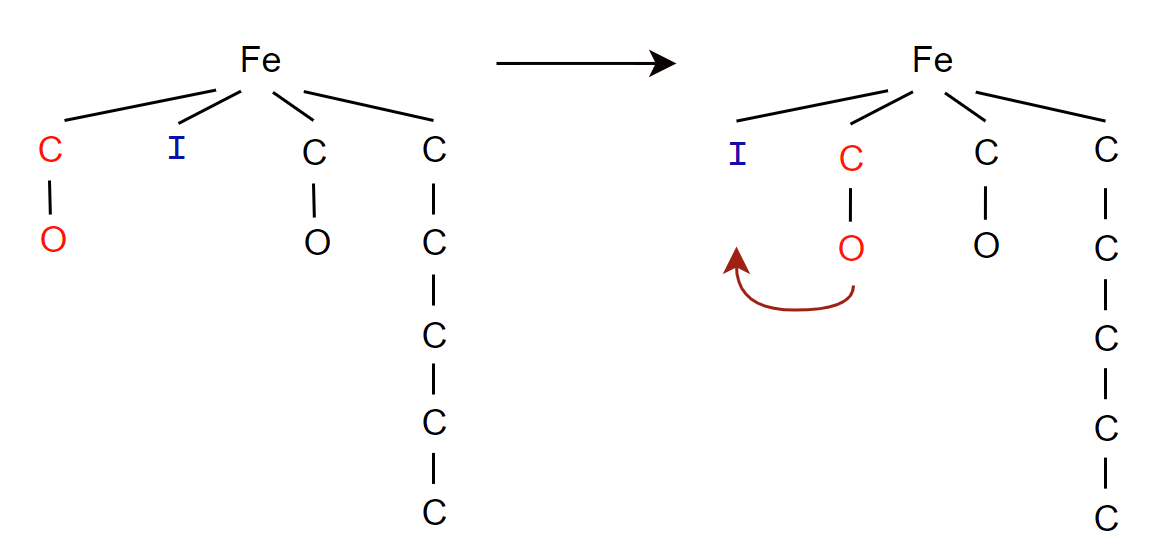
\includegraphics[scale=0.4]{imagenes/diseno/canonizado/rearrange.png}
    \caption{Reordenación de los hijos en función de la longitud de sus ramas. Imagen de elaboración propia. Molécula 28 del Anexo \ref{apend:pagina_tabla_intro_grande}.}
    \label{fig:rearrangeTree}
\end{figure}

En la Figura \ref{fig:desempate_metales1} se muestra el caso para el SMILES 

\begin{center}
\textit{[Cl-][Au+][P](C=1C=CC=CC1)(C=2C=CC=CC2) [C-]34[CH]5=[CH]6[CH]7=[CH]3 [Fe+2]6789\%10\%1154[CH]=\%12[CH]\%11=[CH]\%10 [C-]9([CH]\%128)[P](C)C}
    
\end{center}

el cual tiene 2 metales: un átomo de hierro (Fe) y un átomo de oro (Au). Vemos los 2 árboles generados durante el proceso de selección: en el de la izquierda el hierro se coloca como nodo raíz y se evalúa el subárbol del oro, obteniendo 2 nodos (marcados en rojo); en el de la derecha el oro se coloca como nodo raíz y se evalúa el subárbol del hierro, obteniendo 22 nodos. Se escogerá por tanto el hierro como nodo raíz al tener más nodos que dependen de él. Notar que estos no son los árboles canónicos finales, sino árboles auxiliares cuyo único propósito es seleccionar el primer átomo. Observar también que a ninguno de los dos árboles se le ha aplicado el reordenamiento comentado antes.


\begin{figure}[h!]
\centering
\begin{subfigure}{.5\textwidth}
  \centering
  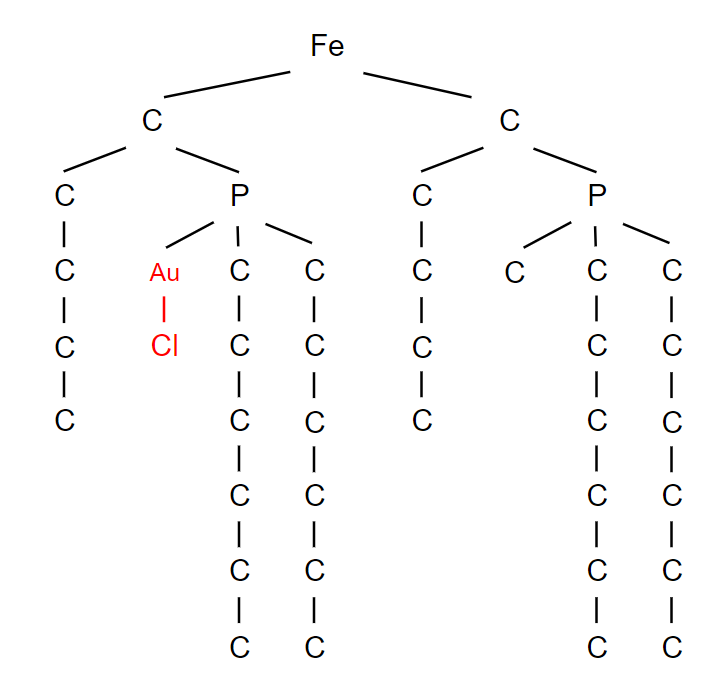
\includegraphics[width=.95\linewidth]{imagenes/diseno/canonizado/mol23Modified_Fe_raiz_resalte.png}
  \caption{}
  \label{fig:sub1}
\end{subfigure}%
\begin{subfigure}{.5\textwidth}
  \centering
  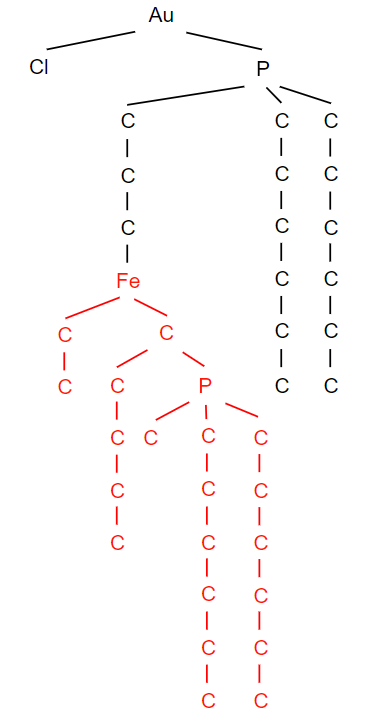
\includegraphics[width=.45\linewidth]{imagenes/diseno/canonizado/mol23Modified_Au_raiz_resalte.png}
  \caption{}
  \label{fig:sub2}
\end{subfigure}
\caption{Esquemas de los árboles generados para la selección del metal. Imagen de elaboración propia. \textbf{(a)} árbol con el hierro como raíz, el subárbol del oro solamente tiene 2 nodos; \textbf{(b)} árbol con el oro como raíz, el subárbol del hierro tiene 22 nodos. Imagen de elaboración propia.}
\label{fig:desempate_metales1}
\end{figure}



\subsection{Sistema de representación 2D} \label{implementacion:dibujado}

Al generar representaciones 2D de una molécula pueden surgir muchas dificultades relacionadas con la disposición de los átomos como su orientación o intentar evitar el solapamiento; y relacionadas con el texto, tipo y tamaño de letra, uso o no de abreviaturas, alineación y posición relativa de las etiquetas con respecto a los demás átomos, etc. Estos problemas se pueden superan de mejor o peor manera mediante una serie de algoritmos, pero por ahora, ninguno es tan versátil como para ajustarse a cualquier tipo de estructura química \cite{david_molecular_2020}. Para más detalles y ejemplos de algoritmos de representación 2D y sus limitaciones en diferentes toolkits (RDKit, OpenBabel, CDK, Avalon e Indigo), se recomienda ver la presentación de 2016 de John Mayfield \cite{comparative_depictions}.

En lo que respecta a este proyecto, se han llevado a cabo 2 modificaciones en el sistema de visualización de OpenBabel para representar moléculas:
\begin{enumerate}
    \item Se ha aumentado la longitud de los enlaces entre átomos para una mayor claridad y separación. Para moléculas organometálicas, en donde un mismo átomo normalmente tiene varios enlaces y existen muchos ciclos, el mero hecho de espaciar un poco los enlaces ya ayuda a que no se vea todo tan unido.
    \item Se han centrado los esfuerzos en la detección y mejora de visualización de estructuras tipo ciclopentadienilo (Cp), muy comunes en organometálica (ver Sección \ref{teoria:ogm}).
\end{enumerate}


Para el segundo punto, se han visualizado una gran cantidad de moléculas que contienen Cp para averiguar las maneras más frecuentes en las que se suelen describir y visualizar. Exsiten varias maneras de representar compuestos de coordinación con ligandos Cp usando enlaces convencionales (Figura \ref{fig:ferrocene_options}), pero ninguna opción refleja correctamente las propiedades de este tipo de uniones.
\begin{figure}[h!]
    \centering
    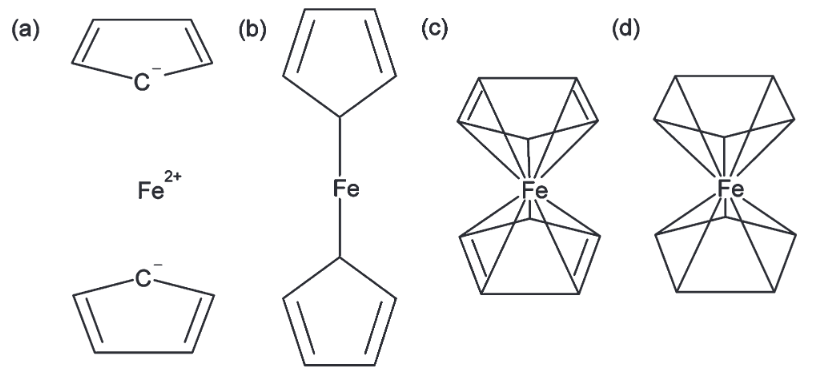
\includegraphics[scale=0.5]{imagenes/diseno/dibujo/varios_intentos_ferroceno.png}
    \caption{Intentos para representar el ferroceno usando enlaces convencionales. \textbf{(a)} ni si quiera representa los enlaces, dibujando varios fragmentos desconectados; \textbf{(b)} mantiene intactos los recuentos de valencia orgánica, desconectando los carbono de enlaces dobles; \textbf{(c)} Ignora las restricciones de valencia normales e incluye todos los enlaces átomo-átomo posibles; \textbf{(d)} representa todos los enlaces significativos a costa de los dobles enlaces. Imagen y descripción extraída y traducida de \cite{zero_order}}
    \label{fig:ferrocene_options}
\end{figure}

Se han valorado otras opciones ya existentes en la literatura, como lo que propone Alex M. Clark en la publicación \textit{``Accurate Specification of Molecular Structures: The Case for Zero-Order Bonds and Explicit Hydrogen Counting"} \cite{zero_order}. Se puede ver en la Figura \ref{fig:zero_bond_ferrocene} el resultado de su propuesta usando lo que él llama enlaces de orden cero (zero-order bonds). 
\begin{figure}[h!]
    \centering
    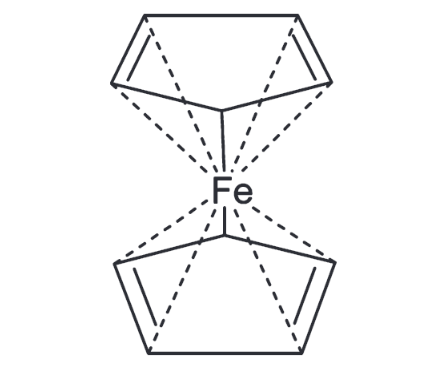
\includegraphics[scale=0.4]{imagenes/diseno/dibujo/zero_bond_orders_ferrocene.png}
    \caption{Ferroceno utilizando enlaces de orden cero según Alex M. Clark. Imagen extraída de \cite{zero_order}.}
    \label{fig:zero_bond_ferrocene}
\end{figure}

Aun así, no se diferencia mucho de la Figura \ref{fig:ferrocene_options}(c) y tampoco termina de ajustarse a cómo los químicos suelen representarlos. Se ha intentado seguir por tanto el manual de la IUPAC \textit{"Graphical representation standards for chemical structure diagrams (IUPAC Recommendations 2008)"}\cite{iupac_manual}, que alberga una gran cantidad de casuísticas con todos los aspectos relacionados a la representación gráfica de la estructura molecular, explicadas de manera detallada y rigurosa. Concretamente en las secciones GR-1.7.1 y GR-6 del manual habla sobre los enlaces de coordinación y enlaces de ciclos aromáticos y electrones deslocalizados. Con lo anterior y atendiendo a las recomendaciones de la experta, el objetivo es implementar la forma mostrada en la Figura \ref{fig:metalocenos_ejemplos}(a) ya que capta la aromaticidad y geometría de los enlaces del ligando.


A todo lo anterior se nos suma el concepto de percepción de anillos, una problemática para nada trivial y que ha estado siempre presente en en mundo de las chemoinformatics. Para entender esto, imaginemos que tenemos una molécula con un anillo de \textit{decalina} (10 carbonos). A la hora de identificar y almacenar la pertenencia a ciclos de cada uno de los átomos no podemos simplemente utilizar todas las combinaciones de ciclos existentes (Figura \ref{fig:decalina_all_ciclos}), ya que haría que un conjunto de átomos pertenezcan simultáneamente a varios anillos (en este caso los átomos 4 y 5). Ejemplo extraído de \cite{sssr_smallest_2020}. Esto según las necesidades de cada aplicación puede suponer un problema o no.

\begin{figure}[h!]
    \centering
    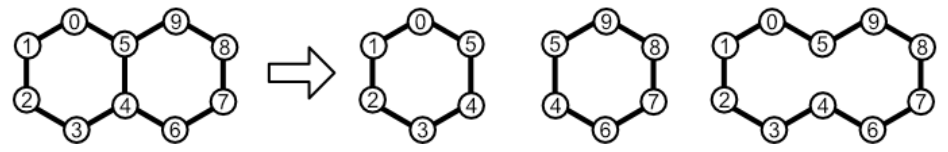
\includegraphics[scale=0.5]{imagenes/diseno/dibujo/decalina_all_cycles.png}
    \caption{Decalina y todo su subset de ciclos.}
    \label{fig:decalina_all_ciclos}
\end{figure}

Por lo general, los algoritmos en los toolkits de chemoinformatics requieren un set de ciclos filtrado, únicamente con los ciclos más pequeños y relevantes. Para el caso anterior, bastaría si nos quedáramos solamente con cualquier combinación de 2 de los 3 ciclos, teniendo así todo el espacio de ciclos cubierto. Esto se puede alcanzar con el algoritmo de SSSR (Smallest Set of Smallest Rings), siendo el que más se usa hoy día para la percepción de anillos \cite{sssr_smallest_2020, sssr_harmful,sssr_counterexamples_2004, sssr_review_1989}. 

La percepción SSSR es la que utiliza OpenBabel y por lo general funciona bien para cualquier tipo de molécula. Pero justamente a la hora de representar estructuras Cp, la forma en la que los átomos de carbono se unen con el metal hace que se genere un conjunto de ciclos que dificulta los algoritmos de detección. Se ilustra este problema con la Figura \ref{fig:sssr_iron(II)}. Supongamos que un hierro (Fe) se une con un ligando Cp. Vemos que cada par de carbonos forma un ciclo de tamaño 3 junto con el hierro, desapareciendo el ciclo original entre los propios carbonos, de manera que internamente tenemos los ciclos almacenados como ``3-1-2, 4-1-3, 5-1-6, 6-1-2 y 5-1-4". Por defecto OpenBabel trata los enlaces como en la Figura \ref{fig:ferrocene_options}(c) y teniendo en cuenta el tratamiento de los ciclos, en la mayoría de casos obtenemos resultados como los de la Figura \ref{fig:iron(II)Original}, ya que a la hora de colocar las líneas de los enlaces, los toma como anillos independientes.

\begin{figure}[h!]
    \centering
    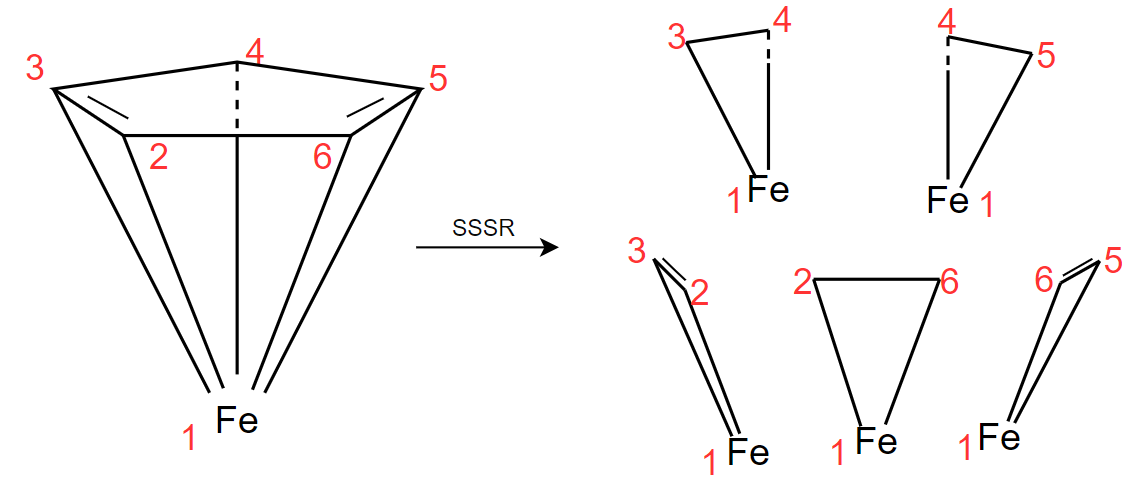
\includegraphics[scale=0.4]{imagenes/diseno/dibujo/sssr_iron.png}
    \caption{Conjunto de ciclos según la percepción SSSR para un hierro con un ligando Cp. Imagen de elaboración propia.}
    \label{fig:sssr_iron(II)}
\end{figure}


\begin{figure}[h!]
    \centering
    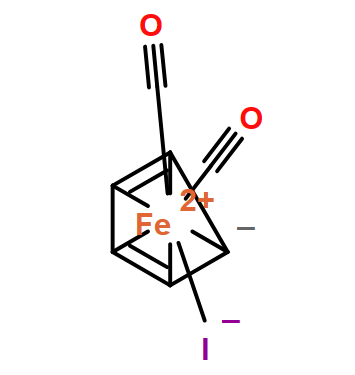
\includegraphics[scale=0.5]{imagenes/diseno/dibujo/iron(II)_Original.png}
    \caption{Representación 2D de la molécula \textit{Dicarbonylcyclopentadienyliodoiron(II)} generada con OpenBabel. Molécula 28 del Anexo \ref{apend:pagina_tabla_intro_grande}.}
    \label{fig:iron(II)Original}
\end{figure}

\subsubsection{Reglas de detección} \label{reglas_deteccion_cp}

Además, hay que tener en cuenta otras situaciones a la hora de detectar Cps completos. Si en la misma molécula hay más de un Cp, cómo se detectan y diferencian cada uno de las estructuras o cómo sabemos qué carbonos forman parte de un Cp o de otro. A través de la cadena SMILES no se puede obtener esa información ya que todos los enlaces son iguales (un metal con un carbono) y la percepción SSSR complicaba más aun la identificación de pertenencia de los carbonos al mismo anillo. En base a esto, surge la identificación por bloques. Se utiliza para esto el árbol canónico explicado previamente con el objetivo identificar relaciones padre-hijo o relaciones de dependencia entre átomos, indicando la pertenencia a una misma subestructura, en este caso a un mismo Cp.

Por tanto, las reglas de detección para una estructura Cp se pueden resumir en:
\begin{itemize}
    \item Que exista un enlace Metal-Carbono
    \item Que el carbono pertenezca a un bloque y que los demás carbonos del mismo bloque tengan también un enlace M-C con el mismo metal que el resto del bloque.
\end{itemize}

Una vez se identifiquen correctamente, se activa un flag especial para marcar qué átomos pertenecen o no a un Cp y darles un tratamiento distinto a la hora de dibujarlos. En concreto:  
\begin{enumerate}
    \item Se crea un único átomo nuevo a modo de señuelo (dummy) para que enlace con el metal.
    \item En base a ese nuevo átomo dummy, se modifican las coordenadas 2D de los carbonos de interés y se disponen en forma de polígono.
    \item Se calcula el círculo central mediante una serie de coordenadas y tanto al círculo como al polígono se le da una perspectiva rotándolos sobre el eje X.
    \item Finalmente se eliminan todos los enlaces M-C para que OpenBabel no los dibuje automáticamente. El hecho de eliminar los enlaces no supone ningún problema ya que no se realizan más operaciones a posteriori que puedan necesitarlos.
\end{enumerate} 

Todo lo relacionado con cada Cp individual se almacena en la clase CpComplex, guardando información como la lista de carbonos que forman el Cp, el metal al que están asociados, el átomo dummy que lo posiciona y el centroide del polígono entre otras cosas.

En el siguiente capítulo se muestran los resultados alcanzados tras la implementación.













